\documentclass{article}
\usepackage[utf8]{inputenc}
\usepackage[hscale=0.7,vscale=0.8]{geometry}

\usepackage{xcolor, listings}
\usepackage{textcomp}
\usepackage{color}

\definecolor{codegreen}{rgb}{0,0.6,0}
\definecolor{codegray}{rgb}{0.5,0.5,0.5}
\definecolor{codepurple}{HTML}{C42043}
\definecolor{backcolour}{HTML}{F2F2F2}
\definecolor{bookColor}{cmyk}{0,0,0,0.90}  
\color{bookColor}

\lstset{upquote=true}

\lstdefinestyle{mystyle}{
	backgroundcolor=\color{backcolour},   
	commentstyle=\color{codegreen},
	keywordstyle=\color{codepurple},
	numberstyle=\numberstyle,
	stringstyle=\color{codepurple},
	basicstyle=\footnotesize\ttfamily,
	breakatwhitespace=false,
	breaklines=true,
	captionpos=b,
	keepspaces=true,
	numbers=left,
	numbersep=10pt,
	showspaces=false,
	showstringspaces=false,
	showtabs=false,
}
\lstset{style=mystyle}

\newcommand\numberstyle[1]{%
	\footnotesize
	\color{codegray}%
	\ttfamily
	\ifnum#1<10 0\fi#1 |%
}

\setlength{\parskip}{1em}

\title{CS-A1153 - Databases, Summer 2020\\
		Project, part 2 (SQL)}
\author{Alberto Nieto Sandino : \href{mailto:alberto.nietosandino@aalto.fi}{alberto.nietosandino@aalto.fi}\\
		Peiyi Zhao : \href{mailto:peiyi.zhao@aalto.fi}{peiyi.zhao@aalto.fi}}
\date{\today}

\usepackage{natbib}
\usepackage{graphicx}
\usepackage{hyperref}

\begin{document}
\begin{titlepage}
	\maketitle
	\vspace{3cm}
	\tableofcontents
	\thispagestyle{empty}
\end{titlepage}

\cleardoublepage

\section{UML diagram}
The following is the UML diagram (Figure \ref{fig:UML}) that we develop for a database given the requirements of the project. Further explanations regarding the diagram and its components are given in the next section.

\begin{figure}[h]
	\centering
	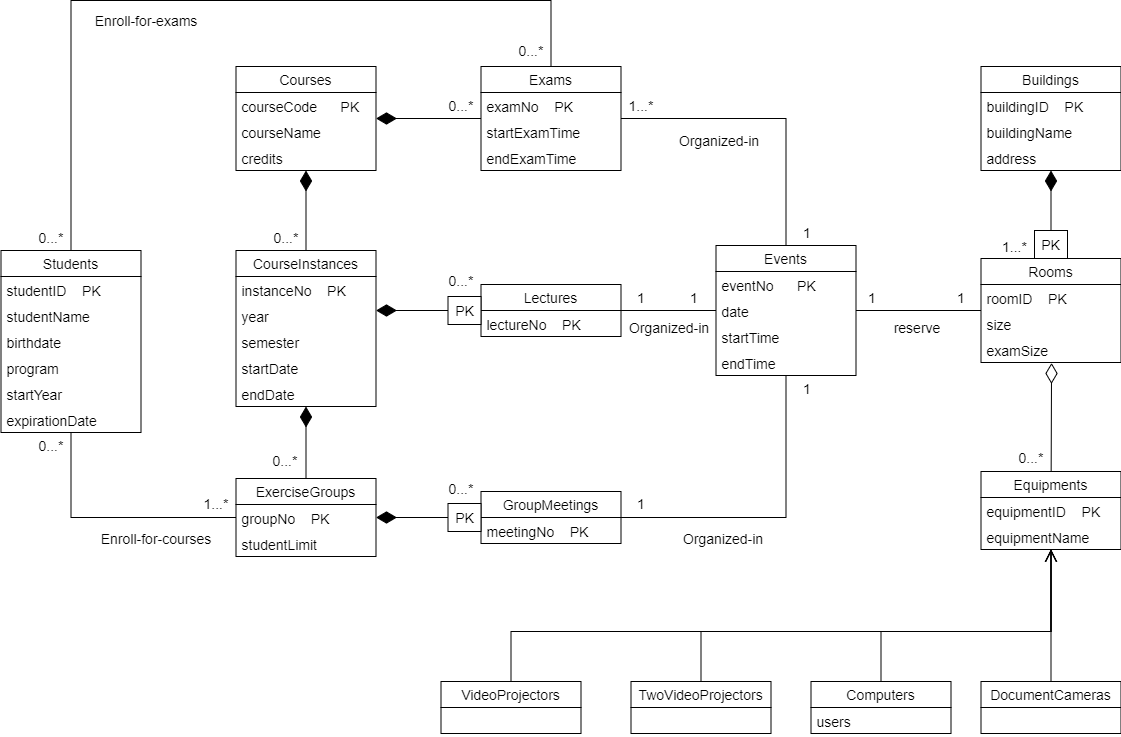
\includegraphics[width=\textwidth]{UML_project_1.png}
	\caption{UML diagram for database}
	\label{fig:UML}
\end{figure}

\section{Relation schema converted from the UML diagram}
Below is the relation schema for the UML diagram of the database.
\begin{itemize}
	\item Courses (\underline{courseCode}, courseName, credits)
	\item CourseInstances (\underline{instanceNo}, year, semester, startDate, endDate, courseCode)
	\item ExerciseGroups (\underline{groupNo}, studentLimit, instanceNo)
	\\\\
	\item Lectures (\underline{instanceNo}, \underline{lectureNo}, eventNo)
	\item GroupMeetings (\underline{groupNo}, \underline{meetingNo}, eventNo)
	\item Exams (\underline{examNo}, startExamTime, endExamTime, courseCode, eventNo)
	\\\\
	\item Students (\underline{studentID}, studentName, birthdate, program, startYear, expirationDate)
	\item Enroll-for-exams (\underline{studentsID}, \underline{examNo})
	\item Enroll-for-courses (\underline{studentID}, \underline{groupNo})
	\\\\
	\item Buildings (\underline{buildingID}, buildingName, address)
	\item Rooms (\underline{buildingID}, \underline{roomID}, size, examSize)
	\\\\
	\item Events (\underline{eventNo}, date, startTime, endTime)
	\item Reserve (eventNo, buildingID, roomID)
	\\\\
	\item Equipments (\underline{equipmentID}, equipmentName, buildingID, roomID)
	\item VideoProjectors (equipmentID)
	\item TwoVideoProjectors (equipmentID)
	\item Computers (equipmentID, users)
	\item DocumentCameras (equipmentID)
\end{itemize}

\section{Explanations}

Courses is a class including the common information for one course like code, name, and
credits. CourseInstances has the basic information about each course implementation. It is
part of the Courses, and it could not exist without Courses, so the relationship between them
is composition. So does ExerciseGroup.

Exams belongs to Courses. Lectures belongs to CourseInstances. GroupMeetings belongs to
ExerciseGroups. All the relationship between these three pairs is many-one relationship.

Events is a class to record the time information when some activity happens in a certain place
at a certain time. So, one lecture or one GroupMeeting could be an event. But several exams
may share an event because they could take place in one room at the same time.

One event could reserve one room. So, there is a one-one association between Events and
Rooms.

Students is a class which stores the information of students. It has two associations. One is
with Exams. The other is with ExerciseGroups. These two associations could be used to
register the course or exam for students.

Rooms is a part of Buildings and could not exist without Buildings. So, the relationship
between them is composition. Equipments is also a part of Rooms, but it can exist without
rooms. So, the relationship between them is aggregation.

VideoProjectors, TwoVideoProjectors and so on are one type of Equipments. So, they are the
subclass of Equipments. And other type of information could be stored in the superclass
Equipments.

The aforementioned UML diagram was designed so as to support a series of queries that were
described in the project requirements. Following is an explanation of how each of these
queries is supported by our designed database.

The database supports storing information about courses, course instances, students,
lectures, exercises groups and their times, exams and enrollments. Courses, course instances,
students, lectures, exercise groups and exams have their own classes where information
about them is stored. Information about the meeting times for exercise groups is stored in
the GroupMeetings class. Enrollments, both for exams and for courses, are represented as
associations:
\begin{itemize}
	\item Enrollment for an exam is an association between the Students and Exams class.
	\item Enrollment for a courses is an association between the Students and ExerciseGroups.
\end{itemize}

The database supports storing information about buildings, rooms and their reservations.
Buildings and rooms store their information in the Buildings classes and Rooms classes
separately. The class Events contains the date and time information of every activity including
exams, lectures and group meetings. Each event has a unique EventNo. If several exams take
place at the same time in one room, they will be regarded as one event and get the same
eventNo. By joining the class Events and the class Reserve, we could find a certain event
reserves a certain room in a certain time. includes reservations for exams, reservations for
lectures and reservation for group meetings.

Courses are composed of the classes Exams and CourseInstances. A CourseInstances class is
a given course organized in a certain semester. Each course instance has a unique instance
number so that it could be recognized even if there are several course instances for the same
course in one semester. Each of these course instances is composed of ExerciseGroups and
Lectures. ExerciseGroups are composed of GroupMeetings which is associated with Events.
Lectures is associated with events. These two latter associations make it possible to keep track
of when a certain lecture or group meeting from a given course instance of a course took
place or will take place at a specific time and date.

If we look at a certain time interval in events, we can have multiple lectures of different course
instances and multiple group meetings of different exercise groups at the same time as long
as their roomID is different. This is shown as the association reserve between Events and
Rooms. Thus, for a given time interval, we can look up which courses have a lecture
reservation in the Events class.

Through the association between Exams and Events, we can see which exams (of a given
Course) take place at a certain time interval. In the Exams class, it is specified the officialduration of the exam (start and end), while in the reservation in Events, the time is longer
since there is a need for practical arrangements both before and after the exam.
In order to see when a certain course will or has been arranged, one can look up the course
instance class. Since course is composed of course instance, it is possible to look up a certain
course code (foreign key in courseInstance which references the primary key in the class
Courses) and see the year and semester when course instances of that course may be taking
place.

Course instances are composed of Lectures and Exercise groups. Thus, it is straightforward to
look up which lectures are associated with which course instances.

Course instances are also composed of Exercised groups, thus we can search which groups
belong to which course instance. Many exercise groups are possible for one course instance.

Once the exercise group is fixed, we can get the eventNo and find the time when this group
meets by looking at Group meetings and its association with events. Through checking the
eventNo in the class Reserve, we can find which room (in a certain building) the group meeting
is taking place in.

To select a room with a certain number of seats and free at a certain time. We can first filter
the Rooms class for rooms with a certain size (i.e. the number of seats). Then, through its
association with Events, we can look at which times these selected rooms are not booked.

If we have a certain roomID with buildingID and a start and end time of a reservation from
Events, we can look up if that corresponds to an exam, a lecture or group meeting (i.e. an
exercise group) by joining these latter 3 classes with that time slot and seeing if there are any
tuples in common. That is tuples where that would be associated with that time slot and
room.

Enrolling of students take place with two associations:
\begin{itemize}
	\item Association Enroll-for-courses which enrols the Student class into the ExerciseGroup,
	thus automatically signing up for a certain course.
	\item Association Enroll-for-exams which enrols the Student class into the Exam for a certain
	Course.
\end{itemize}

To list all students enrolled in a course instance, we can list all of the students who are
enrolled in exerciseGroups of that certain course instance. To list all students enrolled in an
exercise group, we can list the students present in that certain Exercise group (with unique
groupNo). To list all students enrolled in an exam, we can use the Enroll-for-exams association
where each student is associated with a unique exam.


To see if a certain ExerciseGroup is full, we can inspect its studentLimit attribute and count
the tuples grouped by the groupNo. By comparing these two numbers, we could see whether
the limit has been reached or if more students can be enrolled into that ExerciseGroup.

\section{Normal form and functional	dependencies}

The following are the functional dependencies from our database.
\begin{itemize}
	\item courseCode $\rightarrow$ courseName credits
\item instanceNo $\rightarrow$ year semester startDate endDate courseCode
\item groupNo $\rightarrow$ studentLimit instanceNo
\item instanceNo lectureNo $\rightarrow$ eventNo
\item groupNo meetingNo $\rightarrow$ eventNo
\item examNo $\rightarrow$ startExamTime endExamTime courseCode eventNo
\item studentID $\rightarrow$ studentName birthdate program startYear expirationDate
\item buildingID $\rightarrow$ buildingName address
\item buildingID roomID $\rightarrow$ size examSize
\item eventNo $\rightarrow$ date startTime endTime
\item equipmentID $\rightarrow$ equipmentName buildingID roomID
\end{itemize}
Because all the left side is a super key of the relation, it is in BCNF.

\section{Relation schema in SQL}

\begin{lstlisting}[ language=SQL]
CREATE TABLE Courses (
	courseCode TEXT PRIMARY KEY,
	courseName TEXT NOT NULL,
	credits    REAL CHECK (credits > 0) 
);

CREATE TABLE CourseInstances (
	instanceNo TEXT    PRIMARY KEY,
	year       INTEGER CHECK (year > 2000),
	semester   INTEGER CHECK (semester IN (1, 2) ),
	startDate  TEXT,
	endDate    TEXT,
	courseCode TEXT    REFERENCES Courses (courseCode) 
);

CREATE TABLE ExerciseGroups (
	groupNo      TEXT    PRIMARY KEY,
	studentLimit INTEGER CHECK (studentLimit > 0),
	instanceNo   TEXT    REFERENCES CourseInstances (instanceNo) 
);

CREATE TABLE Events (
	eventNo   TEXT PRIMARY KEY,
	date      TEXT,
	startTime TEXT,
	endTime   TEXT
);

CREATE TABLE Lectures (
	instanceNo TEXT,
	lectureNo  TEXT,
	eventNo    TEXT UNIQUE,
	PRIMARY KEY (
		instanceNo,
		lectureNo
	),
	FOREIGN KEY (instanceNo)
	REFERENCES CourseInstances (instanceNo),
	FOREIGN KEY (eventNo)
	REFERENCES Events (eventNo) 
);

CREATE TABLE GroupMeetings (
	groupNo   TEXT,
	meetingNo TEXT,
	eventNo   TEXT UNIQUE,
	PRIMARY KEY (
		groupNo,
		meetingNo
	),
	FOREIGN KEY (groupNo)
	REFERENCES ExerciseGroups (groupNo),
	FOREIGN KEY (eventNo)
	REFERENCES Events (eventNo) 
);

CREATE TABLE Exams (
	examNo        TEXT PRIMARY KEY,
	startExamTime TEXT,
	endExamTime   TEXT,
	courseCode    TEXT NOT NULL,
	eventNo       TEXT NOT NULL,
	FOREIGN KEY (courseCode)
	REFERENCES Courses (courseCode),
	FOREIGN KEY (eventNo)
	REFERENCES Events (eventNo) 
);

CREATE TABLE Students (
	studentID      TEXT    PRIMARY KEY,
	studentName    TEXT,
	birthdate      TEXT,
	program        TEXT,
	startYear      INTEGER,
	expirationDate TEXT
);

CREATE TABLE EnrollForExams (
	studentID TEXT,
	examNo    TEXT,
	PRIMARY KEY (
		studentID,
		examNo
	),
	FOREIGN KEY (studentID)
	REFERENCES Students (studentID),
	FOREIGN KEY (examNo)
	REFERENCES Exams (examNo) 
);

CREATE TABLE EnrollForCourses (
	studentID TEXT,
	groupNo   TEXT,
	PRIMARY KEY (
		studentID,
		groupNo
	),
	FOREIGN KEY (studentID)
	REFERENCES Students (studentID),
	FOREIGN KEY (groupNo)
	REFERENCES ExerciseGroups (groupNo) 
);

CREATE TABLE Buildings (
	buildingID   TEXT PRIMARY KEY,
	buildingName TEXT,
	address      TEXT UNIQUE
);

CREATE TABLE Rooms (
	buildingID TEXT,
	roomID     TEXT,
	size       INTEGER,
	examSize   INTEGERR,
	PRIMARY KEY (
		buildingID,
		roomID
	),
	FOREIGN KEY (
		buildingID
	)
	REFERENCES Buildings (buildingID),
	CHECK (size >= examSize) 
);

CREATE TABLE Equipments (
	equipmentID   TEXT PRIMARY KEY,
	equipmentName TEXT NOT NULL,
	buildingID    TEXT,
	roomID        TEXT,
	FOREIGN KEY (
		buildingID,
		roomID
	)
	REFERENCES Rooms (buildingID,
	roomID) 
);

CREATE TABLE VideoProjectors (
	equipmentID TEXT PRIMARY KEY,
	FOREIGN KEY (equipmentID)
	REFERENCES Equipments (equipmentID) 
);

CREATE TABLE TwoVideoProjectors (
equipmentID TEXT PRIMARY KEY,
FOREIGN KEY (equipmentID)
REFERENCES Equipments (equipmentID) 
);

CREATE TABLE Computers (
	equipmentID TEXT PRIMARY KEY,
	users       TEXT NOT NULL,
	FOREIGN KEY (equipmentID)
	REFERENCES Equipments (equipmentID) 
);

CREATE TABLE DocumentCameras (
	equipmentID TEXT PRIMARY KEY,
	FOREIGN KEY (equipmentID)
	REFERENCES Equipments (equipmentID) 
);

CREATE TABLE Reserve (
	eventNo    TEXT UNIQUE,
	buildingID TEXT NOT NULL,
	roomID     TEXT NOT NULL,
	FOREIGN KEY (eventNo)
	REFERENCES Events (eventNo),
	FOREIGN KEY (
		buildingID,
		roomID
	)
	REFERENCES Rooms (buildingID,
	roomID) 
);
\end{lstlisting}

\section{Insert data into the database}

\begin{lstlisting}[language=SQL]
INSERT INTO Courses
VALUES ('CS-A1150', 'Databases', 5);

INSERT INTO CourseInstances
VALUES ('CS-A1150-2020-1', 2020, 1, '2020-09-03', '2020-11-20', 'CS-A1150');

INSERT INTO ExerciseGroups
VALUES ('CS-A1150-group1', 10, 'CS-A1150-2020-1');

INSERT INTO Events
VALUES ('20200903L1', '2020-09-03', '09:00', '12:00');

INSERT INTO Events
VALUES ('20200904M1', '2020-09-04', '10:00', '11:00');

INSERT INTO Events
VALUES ('20201125E1', '2020-11-25', '08:30', '09:30');

INSERT INTO Lectures
VALUES ('CS-A1150-2020-1', 'lecture1', '20200903L1');

INSERT INTO Lectures(instanceNo, lectureNo)
VALUES ('CS-A1150-2020-1', 'lecture2');

INSERT INTO GroupMeetings
VALUES ('CS-A1150-group1', 'meeting1', '20200904M1');

INSERT INTO GroupMeetings(groupNo, meetingNo)
VALUES ('CS-A1150-group1', 'meeting2');

INSERT INTO Exams
VALUES ('CS-A1150-exam1', '08:40', '09:30', 'CS-A1150', '20201125E1');

INSERT INTO Students
VALUES ('112233', 'Teemu Teekkari', '1990-05-11', 'TIK', '2017', '2021-08-30');

INSERT INTO Students
VALUES ('123456', 'Tiina Teekkari', '1992-09-23', 'TUO', '2019', '2023-08-30');

INSERT INTO Students
VALUES ('224411', 'Maija Virtanen', '1991-12-05', 'AUT', '2018', '2022-08-30');

INSERT INTO EnrollForExams
VALUES ('112233', 'CS-A1150-exam1');

INSERT INTO EnrollForCourses
VALUES ('112233', 'CS-A1150-group1');

INSERT INTO Buildings
VALUES ('building1', 'Computer Science Building', 'Tietotekniikantalo, 
	Konemiehentie 2, 02150 Espoo');

INSERT INTO Rooms
VALUES ('building1', 'room101', 30, 20);

INSERT INTO Equipments
VALUES ('equipment1', 'MacComputer', 'building1', 'room101');

INSERT INTO Equipments
VALUES ('equipment2', 'SONY VideoProject', 'building1', 'room101');

INSERT INTO VideoProjectors
VALUES ('equipment2');

INSERT INTO Computers
VALUES ('equipment1', 'teachers');

INSERT INTO Reserve
VALUES ('20200903L1', 'building1', 'room101');
\end{lstlisting}

\section{Views}

\begin{lstlisting}[language=SQL]
CREATE VIEW LectureTimePlace AS
	SELECT instanceNo,
		lectureNo,
		date,
		startTime,
		endTime,
		buildingID,
		roomID
	FROM (
		SELECT instanceNo,
			lectureNo,
			Lectures.eventNo,
			date,
			startTime,
			endTime
		FROM Lectures
			LEFT JOIN
			Events ON Lectures.eventNo = Events.eventNo
	)
	AS LectureTime
	LEFT JOIN
	Reserve ON LectureTime.eventNo = Reserve.eventNo;

CREATE VIEW MeetingTimePlace AS
	SELECT groupNo,
		meetingNo,
		date,
		startTime,
		endTime,
		buildingID,
		roomID
	FROM (
		SELECT groupNo,
			meetingNo,
			GroupMeetings.eventNo,
			date,
			startTime,
			endTime
		FROM GroupMeetings
			LEFT JOIN
			Events ON GroupMeetings.eventNo = Events.eventNo
	)
	AS MeetingTime
	LEFT JOIN
	Reserve ON MeetingTime.eventNo = Reserve.eventNo;

CREATE VIEW ExamTimePlace AS
	SELECT courseCode,
		examNo,
		startExamTime,
		endExamTime,
		date,
		startTime,
		endTime,
		buildingID,
		roomID
	FROM (
		SELECT courseCode,
			examNo,
			Exams.eventNo,
			startExamTime,
			endExamTime,
			date,
			startTime,
			endTime
		FROM Exams
			LEFT JOIN
			Events ON Exams.eventNo = Events.eventNo
	)
	AS ExamTime
	LEFT JOIN
	Reserve ON ExamTime.eventNo = Reserve.eventNo;
\end{lstlisting}

\section{Indexes}

\section{Use cases}
\begin{lstlisting}[language=SQL]
/* Query the exact number and the limit number of students in one group */
SELECT EnrollForCourses.groupNo, COUNT(studentID), studentLimit
FROM EnrollForCourses, ExerciseGroups
WHERE EnrollForCourses.groupNo = ExerciseGroups.groupNo
Group BY EnrollForCourses.groupNo

/* Query the exact number of students in one exam */
SELECT examNo, COUNT(studentID)
FROM EnrollForExams
GROUP BY examNo

/* Query the number of computers in one room which could used by students to have a lecture or exam */
SELECT buildingID, roomID, COUNT(Computers.equipmentID)
FROM Computers, Equipments
WHERE users = 'students' AND Computers.equipmentID = Equipments.equipmentID 
GROUP BY buildingID, roomID
\end{lstlisting}
\end{document}
